\documentclass[10pt,UTF8]{ctexart}


\usepackage[margin=2cm,a4paper]{geometry}
%\usepackage[left=0.75in,top=0.6in,right=0.75in,bottom=1.0in,a4paper]{geometry}

\setmainfont{Caladea}
%% 也可以選用其它字庫:
% \setCJKmainfont[%
%   ItalicFont=AR PL KaitiM GB,
%   BoldFont=Noto Sans CJK SC,
% ]{Noto Serif CJK SC}
% setCJKsansfont{Noto Sans CJK SC}
% \renewcommand{\kaishu}{\CJKfontspec{AR PL KaitiM GB}}

% 繁體中文
\setCJKmainfont[Path=fonts/ ]{NotoSansTC-Medium.otf}

\usepackage{minted}
\usepackage[breaklinks]{hyperref}

% Picture
% 導言區的此三行無變化
\usepackage{graphicx}
\usepackage{float} 
\usepackage{subfigure}
% 以下是新增的自定義格式更改
\usepackage[]{caption2} %新增調用的宏包
\renewcommand{\figurename}{Fig.} %重定義編號前綴詞
\renewcommand{\captionlabeldelim}{.~} %重定義分隔符
 %\roman 是羅馬數字編號,\alph是默認的字母編號,\arabic是阿拉伯數字編號,可按需替換下一行的相應位置
\renewcommand{\thesubfigure}{(\roman{subfigure})}%此外,還可設置圖編號顯示格式,加括號或者不加括號
\makeatletter \renewcommand{\@thesubfigure}{\thesubfigure \space}%子圖編號與名稱的間隔設置
\renewcommand{\p@subfigure}{} \makeatother

% Math
\usepackage {mathtools}
\usepackage{amssymb}

% Code
\usepackage{listings}
\usepackage{xcolor}
\lstset{
    % backgroundcolor=\color{red!50!green!50!blue!50},
    % 程式碼塊背景色為淺灰色
    rulesepcolor= \color{gray}, % 程式碼塊邊框顏色
    breaklines=true,  % 程式碼過長則換行
    numbers=left, % 行號在左側顯示
    numberstyle= \small,% 行號字型
    % eywordstyle= \color{red,% 關鍵字顏色
    commentstyle=\color{gray}, % 註釋顏色
    frame=shadowbox % 用方框框住程式碼塊
    }

\usepackage{hyperref}

\title{算法分析和複雜性理論}
\author{干皓丞,2101212850, 信息工程學院}

\begin{document}
\maketitle


\section{作業目標與章節摘要}

1. LeetCode 56. Merge Intervals 合併區間

2. LeetCode 148. Sort List 排序鍊錶

3. LeetCode 274. H-Index, H 指數


\section{作業內容概述}

作業可以從 GitHub 下的 kancheng/kan-cs-report-in-2022 專案找到,作業程式碼與文件目錄為 kan-cs-report-in-2022/AATCC/lab-report/w3。實際執行的環境與實驗設備為 Google 的 Colab 、MacBook Pro (Retina, 15-inch, Mid 2014) 、 Acer Aspire R7 與 HP Victus (Nvidia GeForce RTX 3060)。

本作業 GitHub 專案為 kancheng/kan-cs-report-in-2022 下的 AATCC` 的目錄。程式碼可以從 code 目錄下可以找到 *.pynb,內容包含上次課堂練習、LeetCode 範例思路整理與作業。

https://github.com/kancheng/kan-cs-report-in-2022/tree/main/AATCC

\begin{figure}[H]
\centering 

\includegraphics[width=0.30\textwidth]{aatccqr.png} 
\caption{作業專案位置}
\label{Test}
\end{figure}


1. LeetCode : https://leetcode.com/

2. LeetCode CN : https://leetcode-cn.com/

3. OnlineGDB : https://www.onlinegdb.com/ 

LeetCode 的平台部分, CN 的平台有針對簡體中文使用者進行處理,包含中英文切換等功能。OnlineGDB 則可線上進行簡易的環境測試,其程式碼涵蓋 C, C++, C\#, Java, Python, JS, Rust, Go。

\newpage

\section{LeetCode 56. Merge Intervals 合併區間}

\subsection{LeetCode 56. 題目}

Given an array of intervals where intervals[i] = [$start_{i}, end_{i}$], merge all overlapping intervals, and return an array of the non-overlapping intervals that cover all the intervals in the input.

以數組 intervals 表示若干個區間的集合,其中單個區間為 intervals[i] = [$start_{i}, end_{i}$] 。請你合併所有重疊的區間,並返回 一個不重疊的區間數組,該數組需恰好覆蓋輸入中的所有區間。

Example 1:

\begin{lstlisting}[language={python}]
Input: intervals = [[1,3],[2,6],[8,10],[15,18]]
Output: [[1,6],[8,10],[15,18]]
Explanation: Since intervals [1,3] and [2,6] overlaps, merge them into [1,6].
\end{lstlisting}

Example 2:

\begin{lstlisting}[language={python}]
Input: intervals = [[1,4],[4,5]]
Output: [[1,5]]
Explanation: Intervals [1,4] and [4,5] are considered overlapping.
\end{lstlisting}

Constraints:

1. 1 <= intervals.length <= $10^4$

2. intervals[i].length == 2

3. 0 <= $start_{i}$ <= $end_{i}$ <= $10^4$

\subsection{LeetCode 56. 思路總結}

先按照區間起點進行排序。然後從區間起點小的開始掃描,依次合併每個有重疊的區間。

\subsection{LeetCode 56. Code 範例}

LeetCode 56. Python 

\begin{lstlisting}[language={python}]
from typing import List
class Solution:
    def merge(self, intervals: List[List[int]]) -> List[List[int]]:
        intervals.sort()
        ans = [intervals[0]]
        L, R = 1, 0
        while L < len(intervals):
            if ans[R][1] < intervals[L][0]:
                ans.append(intervals[L])
                L += 1
                R += 1
            else:
                ans[R] = [ans[R][0], max(ans[R][1], intervals[L][1])]
                L += 1
        return ans
\end{lstlisting}

\subsection{LeetCode 56. 結果}

\begin{figure}[H]
\centering 
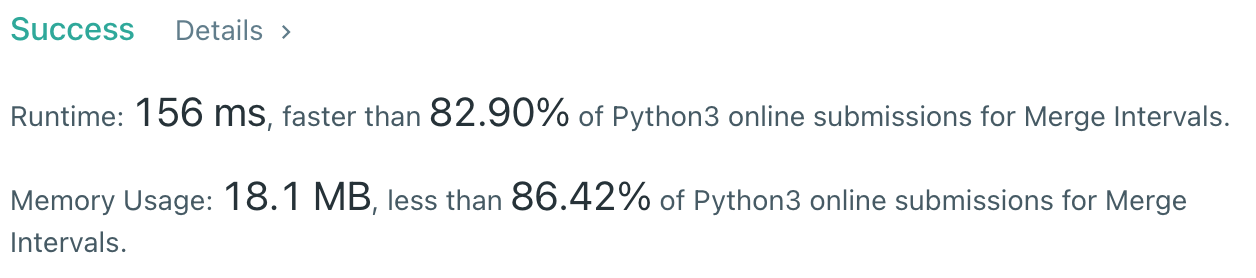
\includegraphics[width=0.80\textwidth]{lc-56-o.png} 
\caption{LeetCode 56 結果}
\label{Test}
\end{figure}


\newpage

\section{LeetCode 148. Sort List 排序鍊錶}

\subsection{LeetCode 148. 題目}

Given the head of a linked list, return the list after sorting it in ascending order.

給你鍊錶的頭結點 head ,請將其按 升序 排列並返回 排序後的鍊錶。

\begin{figure}[H]
\centering 
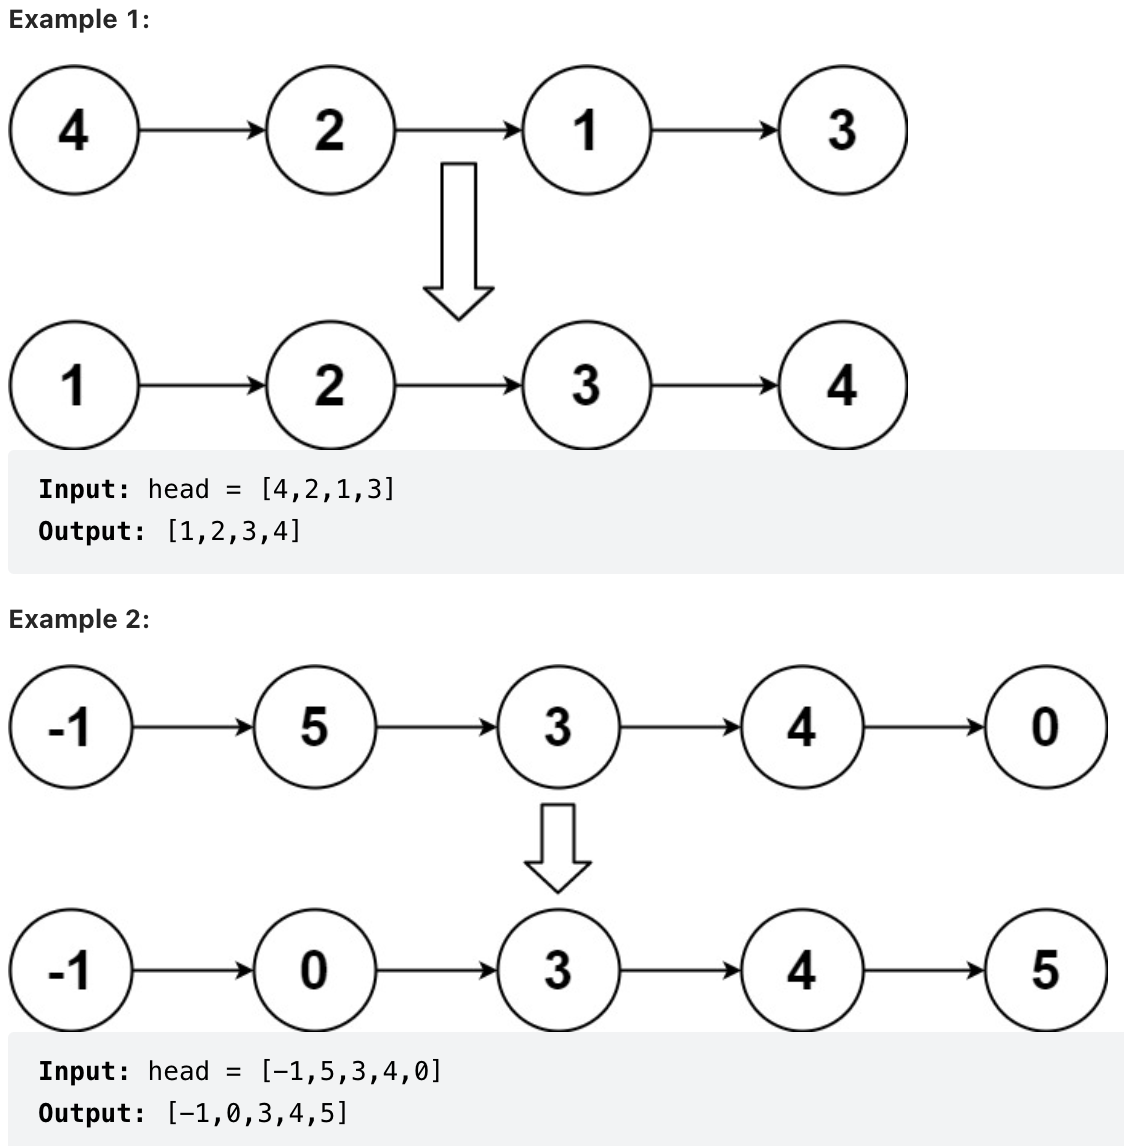
\includegraphics[width=0.80\textwidth]{lc-148-example.png} 
\caption{Example}
\label{Test}
\end{figure}

Example 1:

\begin{lstlisting}[language={python}]
Input: head = [4,2,1,3]
Output: [1,2,3,4]
\end{lstlisting}

Example 2:

\begin{lstlisting}[language={python}]
Input: head = [-1,5,3,4,0]
Output: [-1,0,3,4,5]
\end{lstlisting}

Example 3:
\begin{lstlisting}[language={python}]
Input: head = []
Output: []
\end{lstlisting}


Constraints:

1. The number of nodes in the list is in the range [0, 5 * $10^4$].(鍊錶中節點的數目在範圍 [0, 5 * $10^4$])

2. $-10^5$ <= Node.val <= $10^5$

Follow up: Can you sort the linked list in O(n logn) time and O(1) memory (i.e. constant space)?

你可以在 O(n log n) 時間複雜度和常數級空間複雜度下,對鍊錶進行排序嗎?

\subsection{LeetCode 148. 思路總結}

歸併排序 ..

\subsection{LeetCode 148. Code 範例}

\begin{lstlisting}[language={python}]
# Definition for singly-linked list.
class ListNode:
    def __init__(self, val=0, next=None):
        self.val = val
        self.next = next

class Solution:
    def sortList(self, head: ListNode) -> ListNode:
        h_head = ListNode(-1, head)
        mem = []
        while(head is not None):
            next_h = head.next
            head.next = None
            mem.append(head)
            head = next_h
        mem = sorted(mem, key=lambda x: x.val)
        n = len(mem)
        if n == 0:
            return None
        h_head.next = mem[0]
        for i in range(n-1):
            mem[i].next = mem[i+1]     
        return h_head.next
\end{lstlisting}

\subsection{LeetCode 148. 結果}

\begin{figure}[H]
\centering 
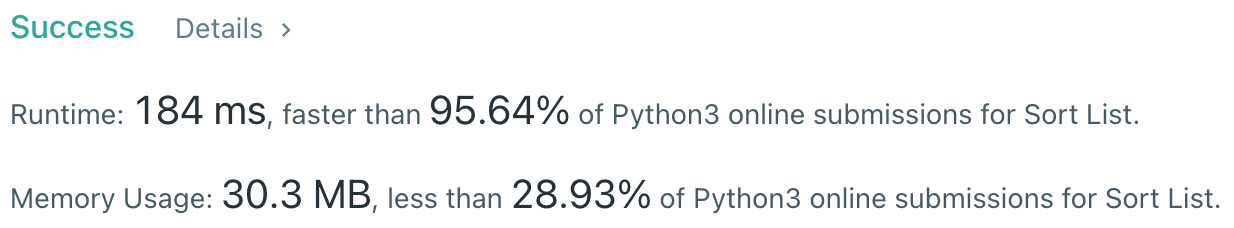
\includegraphics[width=0.80\textwidth]{lc-148-o.png} 
\caption{LeetCode 148 結果}
\label{Test}
\end{figure}


\newpage

\section{LeetCode 274. H-Index, H 指數點}

\subsection{LeetCode 274. 題目}

Given an array of integers citations where citations[i] is the number of citations a researcher received for their ith paper, return compute the researcher's h-index.

According to the definition of h-index on Wikipedia: A scientist has an index h if h of their n papers have at least h citations each, and the other n − h papers have no more than h citations each.

If there are several possible values for h, the maximum one is taken as the h-index.

給你一個整數數組 citations ,其中 citations[i] 表示研究者的第 i 篇論文被引用的次數。計算並返回該研究者的 h 指數。

根據維基百科上 h 指數的定義:h 代表“高引用次數”,一名科研人員的 h指數是指他(她)的 (n 篇論文中)總共有 h 篇論文分別被引用了至少 h 次。且其餘的 n - h 篇論文每篇被引用次數不超過 h 次。

如果 h 有多種可能的值,h 指數 是其中最大的那個。

Example 1:

\begin{lstlisting}[language={python}]
Input: citations = [3,0,6,1,5]
Output: 3
Explanation: [3,0,6,1,5] means the researcher has 5 papers in total and each of them had received 3, 0, 6, 1, 5 citations respectively.
Since the researcher has 3 papers with at least 3 citations each and the remaining two with no more than 3 citations each, their h-index is 3.

給定數組表示研究者總共有 5 篇論文,每篇論文相應的被引用了 3, 0, 6, 1, 5 次。
由於研究者有 3 篇論文每篇 至少 被引用了 3 次,其餘兩篇論文每篇被引用 不多於 3 次,所以她的 h 指數是 3。
\end{lstlisting}

Example 2:
\begin{lstlisting}[language={python}]
Input: citations = [1,3,1]
Output: 1
\end{lstlisting}

Constraints:

1. n == citations.length

2. 1 <= n <= 5000

3. 0 <= citations[i] <= 1000

Follow up: Could you do this in one pass?(你能嘗試使用一趟掃描實現嗎?)

\subsection{LeetCode 274. 思路總結}

可以先將數組裡面的數從小到大排序。因為要找最大的 h-index,所以從數組末尾開始往前找,找到第一個數組的值,小於,總長度減去下標的值,這個值就是 h-index。

\subsection{LeetCode 274. Code 範例}

\begin{lstlisting}[language={python}]
class Solution(object):
    def hIndex(self, citations):
        index = 0
        citations.sort(reverse=True)
        for i in citations:
            if i > index:
                index +=1
        return index
\end{lstlisting}

\subsection{LeetCode 274. 結果}

\begin{figure}[H]
\centering 
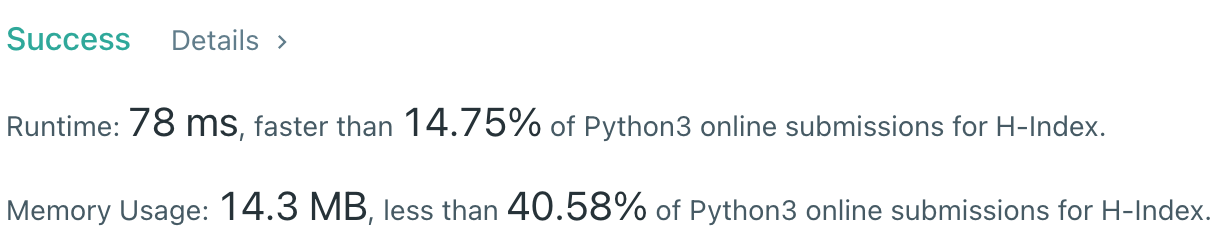
\includegraphics[width=0.80\textwidth]{lc-274-o.png} 
\caption{LeetCode 274 結果}
\label{Test}
\end{figure}




%\section{附錄}

% 數學意義說明

% $$\min \limits_{G}\max \limits_{D}{V_I(D,\ G)=V(D,G)-\lambda L_I(G,Q)}$$

%	\begin{lstlisting}[language={python}]

%	\end{lstlisting}

%\begin{enumerate}
%\item Y
%\item A
%\end{enumerate}

% \newpage

\clearpage

\end{document}